% Provenance (never printed): see sources/outline_sources.md (Year 2: fractional
% crystallisation, Bowen's series, compatible and incompatible elements, mixing and
% assimilation, layered intrusions).
% Curves from figdata/bachelor-2/differentiation.py (Bowen 1913 plagioclase loop, Rayleigh and
% equilibrium laws, Wilcox 1954 Paricutin analyses and mass balance, AFC closed form,
% Tegner et al. 2023 Skaergaard whole-rock data); exercise and problem values in the Book 4
% scratch calculator calc/ch08.py.
\chapter{Diferensiasi Magma}\label{ch:b2:magmatic-differentiation}

Pada 20 Februari 1943 sebuah gunung api mulai meletus di bagian barat Meksiko, dan letusannya berlangsung
selama sembilan tahun. Lava pertamanya adalah andesit basaltik dengan silika \qty{55}{\percent};
lava terakhirnya, pada Februari 1952, adalah andesit dengan silika sedikit di atas
\qty{60}{\percent}. Gunung api itu, Parícutin, tidak berpindah ke sumber lain selama
itu, dan lava-lavanya dianalisis satu demi satu begitu keluar. \omterm{def:b2:magma-emplacement:magma}{Magma}
di bawahnya mengubah dirinya sendiri: \omterm{def:b2:magma-emplacement:magma}{magma} itu menumbuhkan kristal lalu meninggalkannya, dan \omterm{def:b2:magma-emplacement:magma}{magma} itu melahap
sebagian batuan granitik di sekelilingnya. \omterm{def:b2:magma-emplacement:magma}{Magma} yang meninggalkan mantel sebagai basal dapat
berakhir sebagai riolit, dan batuan yang ditinggalkannya di sepanjang jalan merekam bagaimana hal itu terjadi.
Bab ini mengikuti \omterm{def:b2:magma-emplacement:magma}{magma} selama mendingin: urutan mengkristalnya mineral,
hukum-hukum yang menyatakan bagaimana unsur utama dan \omterm{def:b2:elements-in-the-earth:trace}{unsur jejak} berubah ketika kristal disingkirkan,
batuan yang dibangun dari kristal-kristal itu, dan apa yang terjadi ketika \omterm{def:b2:magma-emplacement:magma}{magma} menerima
\omterm{def:b2:magma-emplacement:magma}{magma} lain atau kerak.
% ledger: wilcox54:paricutin

\begin{recall}
\textbf{Dari volume sekolah menengah atas}: batuan beku dan teksturnya; urutan
mengkristalnya mineral dari \omterm{def:b2:magma-emplacement:magma}{magma} basaltik, olivin pertama dan kuarsa terakhir,
yang ditemukan melalui percobaan Bowen. \textbf{Dari volume Tahun 2 buku kimia}:
diagram fase biner, larutan padat, dan aturan tuas. \textbf{Dari volume Tahun
1}: plagioklas, larutan padat antara anortit \ce{CaAl2Si2O8} dan albit
\ce{NaAlSi3O8}, serta silikat pembentuk batuan lainnya; sayatan tipis di antara polarisator
bersilang. \textbf{Dari \cref{ch:b2:elements-in-the-earth}}: \omterm{def:b2:elements-in-the-earth:partition}{koefisien partisi mineral--lelehan} dan
koefisien partisi total, $\bar D = \sum_i x_i D_i$, \omterm{def:b2:elements-in-the-earth:partition}{unsur kompatibel} dan inkompatibel,
\omterm{def:b2:elements-in-the-earth:normalised}{diagram ternormalisasi}, dan \omterm{prop:b2:elements-in-the-earth:normalised}{anomali europium}. \textbf{Dari
\cref{ch:b2:isotope-geochemistry}}: rasio isotop sebagai pelacak dan \omterm{prop:b2:isotope-geochemistry:mixing}{hiperbola
pencampuran}. \textbf{Dari \cref{ch:b2:mantle-melting}}: eutektik diopsid--anortit,
\omterm{def:b2:mantle-melting:peritectic}{pelelehan inkongruen}, diagram terner, dan \omterm{def:b2:mantle-melting:primary}{magma primer}.
\end{recall}

\section{Urutan kristalisasi}\label{sec:b2:magmatic-differentiation:sequences}

\omterm{def:b2:magma-emplacement:magma}{Magma} basaltik tidak mengkristalkan semua mineralnya sekaligus. Melalui percobaan, Bowen menemukan
bahwa olivin biasanya mengkristal pertama, pada suhu antara 1200 dan
\qty{1300}{\celsius}; bahwa plagioklas kaya kalsium mulai mengkristal kira-kira bersamaan dengan
piroksen; dan bahwa cairan terakhir yang kaya silika menghasilkan feldspar kalium, kuarsa, dan
mungkin muskovit pada sekitar 750 sampai \qty{800}{\celsius}. Di antara keduanya, mineral
mafik tidak sekadar menumpuk: masing-masing bereaksi dengan cairan untuk menghasilkan mineral berikutnya.
% ledger: earle:bowen (Book 2), tulane:bowen (Book 2)

\begin{definition}[Seri reaksi Bowen]\label{def:b2:magmatic-differentiation:bowen}
Yang disebut \emph{seri reaksi Bowen}\index{seri reaksi Bowen} adalah urutan
mengkristalnya silikat umum dari \omterm{def:b2:magma-emplacement:magma}{magma} basaltik yang mendingin, berupa dua cabang
yang bertemu di ujungnya. Pada \emph{cabang diskontinu}, setiap mineral mafik
bereaksi dengan cairan membentuk mineral baru dengan struktur lain: olivin,
piroksen, amfibol, biotit. Pada \emph{cabang kontinu}, plagioklas
mengkristal sepanjang waktu, dengan komposisi yang berubah secara kontinu dari kaya kalsium
menjadi kaya natrium. Cairan terakhir mengkristalkan feldspar kalium, muskovit, dan
kuarsa.
\end{definition}
% ledger: earle:bowen (Book 2)

\begin{omfigure}
\centering
\begin{tikzpicture}[font=\small, x=1cm, y=1cm,
  mn/.style={draw, rounded corners=2pt, fill=white, inner sep=3pt, minimum width=2.3cm,
             align=center}]
\draw[-{Stealth[length=4pt]}, thick, gray] (-1.3,0.3) -- (-1.3,-6.0);
\node[rotate=90, anchor=south, font=\scriptsize, gray] at (-1.4,-2.85) {suhu menurun};
\node[anchor=east, font=\scriptsize] at (-1.5,0) {$\approx$ 1200--\qty{1300}{\celsius}};
\node[anchor=east, font=\scriptsize] at (-1.5,-5.6) {$\approx$ 750--\qty{800}{\celsius}};
\node[mn] (ol) at (1,0) {olivin};
\node[mn] (px) at (1,-1.4) {piroksen};
\node[mn] (am) at (1,-2.8) {amfibol};
\node[mn] (bt) at (1,-4.2) {biotit};
\draw[-{Stealth[length=4pt]}, thick] (ol) -- (px);
\draw[-{Stealth[length=4pt]}, thick] (px) -- (am);
\draw[-{Stealth[length=4pt]}, thick] (am) -- (bt);
\node[font=\scriptsize, align=center] at (1,0.8) {cabang diskontinu\\(mineral baru di setiap tahap)};
\node[mn] (ca) at (6,-1.4) {plagioklas\\kaya kalsium};
\node[mn] (na) at (6,-4.2) {plagioklas\\kaya natrium};
\fill[left color=white, right color=white, top color=orange!35, bottom color=orange!8]
  (5.75,-2.0) rectangle (6.25,-3.6);
\draw[-{Stealth[length=4pt]}, thick] (ca) -- (na);
\node[font=\scriptsize, align=center] at (6,0.8) {cabang kontinu\\(satu mineral, komposisi berubah)};
\node[mn, minimum width=7.2cm] (last) at (3.5,-5.6) {feldspar kalium, muskovit, kuarsa};
\draw[-{Stealth[length=4pt]}, thick] (bt) -- (bt|-last.north);
\draw[-{Stealth[length=4pt]}, thick] (na) -- (na|-last.north);
\end{tikzpicture}
\par\smallskip{\small \omterm{def:b2:magmatic-differentiation:bowen}{Seri reaksi Bowen}. Olivin dan plagioklas kaya kalsium
mengkristal paling dulu dari \omterm{def:b2:magma-emplacement:magma}{magma} basaltik; di kiri, setiap mineral mafik bereaksi dengan
cairan untuk menghasilkan mineral berikutnya, di kanan, plagioklas makin lama makin kaya akan
natrium; cairan terakhir yang kaya silika menghasilkan feldspar kalium, muskovit, dan kuarsa.
Suhu yang tertera adalah nilai khas untuk \omterm{def:b2:magma-emplacement:magma}{magma} basaltik pada tekanan rendah.}
\end{omfigure}
% ledger: earle:bowen (Book 2)

Kedua cabang itu bersesuaian dengan dua jenis diagram fase pada
\cref{ch:b2:mantle-melting}. Reaksi diskontinu adalah \omterm{def:b2:mantle-melting:peritectic}{pelelehan inkongruen}
enstatit yang berjalan mundur: kristal forsterit bereaksi dengan cairan yang lebih kaya akan silika untuk
menghasilkan enstatit. Cabang kontinu adalah larutan padat. Bowen mengukurnya pada 1913
pada plagioklas sintetis, dengan menahan setiap komposisi pada suhu yang diketahui lalu
mencari kaca dan kristal: anortit meleleh pada \qty{1550}{\celsius}, albit pada
sekitar \qty{1100}{\celsius}, dan setiap plagioklas antara meleleh dalam suatu selang
di antara kurva bawah, yaitu solidus, dan kurva atas, yaitu likuidus (gambar
di bawah).
% ledger: bowen13:plagioclase, bowen14:mgo-sio2

\begin{omfigure}
\centering
\begin{tikzpicture}
\begin{axis}[omrecord, width=0.78\linewidth, height=6.4cm,
  xmin=0, xmax=100, ymin=1050, ymax=1600,
  xlabel={anortit (\unit{\percent}, molekuler)}, ylabel={suhu (\unit{\celsius})},
  y tick label style={/pgf/number format/1000 sep={}}, unbounded coords=discard,
  tick label style={font=\scriptsize}, label style={font=\small}]
\addplot[very thick, black] table[x=an, y=T_liq] {figdata/out/bachelor-2-differentiation-plag-curve.dat};
\addplot[very thick, black, dashed] table[x=an, y=T_sol] {figdata/out/bachelor-2-differentiation-plag-curve.dat};
\addplot[only marks, mark=*, mark size=1.5pt, blue!70!black] table[x=an, y=T_liq] {figdata/out/bachelor-2-differentiation-plag-data.dat};
\addplot[only marks, mark=o, mark size=1.7pt, blue!70!black] table[x=an, y=T_sol] {figdata/out/bachelor-2-differentiation-plag-data.dat};
\draw[densely dotted, red!70!black, thick] (axis cs:50,1560) -- (axis cs:50,1287);
\draw[red!70!black, thick] (axis cs:50,1450) -- (axis cs:80.6,1450);
\draw[red!70!black, thick] (axis cs:33.3,1394) -- (axis cs:70.6,1394);
\draw[red!70!black, thick] (axis cs:13.9,1287) -- (axis cs:50,1287);
\addplot[only marks, mark=*, mark size=1.4pt, red!70!black] coordinates {(50,1450) (80.6,1450) (33.3,1394) (70.6,1394) (13.9,1287) (50,1287)};
\node[font=\scriptsize] at (axis cs:30,1530) {cairan};
\node[font=\scriptsize, align=center] at (axis cs:83,1200) {plagioklas\\(larutan padat)};
\node[font=\scriptsize, anchor=west] at (axis cs:2,1430) {likuidus (garis penuh)};
\node[font=\scriptsize, anchor=west] at (axis cs:42,1160) {solidus (putus-putus)};
\node[font=\scriptsize, anchor=south, red!70!black, fill=white, inner sep=1pt] at (axis cs:68,1452) {\qty{1450}{\celsius}};
\node[font=\scriptsize, anchor=north, red!70!black, fill=white, inner sep=1pt] at (axis cs:31,1284) {\qty{1287}{\celsius}};
\end{axis}
\end{tikzpicture}
\par\smallskip{\small Feldspar plagioklas pada tekanan atmosfer, dari
percobaan quenching Bowen (1913): awal (lingkaran) dan akhir (titik)
pelelehan, dengan kurva yang ditarik melalui hasil pengukuran. Merah: \omterm{def:b2:magmatic-differentiation:crystallisation}{kristalisasi
setimbang} cairan dengan \qty{50}{\percent} anortit; kristal pertama, pada
\qty{1450}{\celsius}, mengandung \qty{81}{\percent} anortit; pada \qty{1394}{\celsius},
kristal \qty{71}{\percent} berdampingan dengan cairan \qty{33}{\percent}; cairan
terakhir, pada \qty{1287}{\celsius}, mengandung \qty{14}{\percent} (\cref{exo:b2:magmatic-differentiation:1}).}
\end{omfigure}
% ledger: bowen13:plagioclase

Cairan yang mengkristalkan larutan padat menjadi diperkaya oleh komponen yang
meleleh pada suhu lebih rendah: plagioklas pertama dari cairan dengan
\qty{50}{\percent} anortit mengandung \qty{81}{\percent}, dan cairan bergerak ke arah
albit. Apa yang terjadi selanjutnya bergantung pada apakah kristal-kristal itu tetap berinteraksi dengan
cairan.

\begin{definition}[Kristalisasi setimbang dan kristalisasi fraksional]
\label{def:b2:magmatic-differentiation:crystallisation}
Pada \emph{kristalisasi setimbang}\index{kristalisasi setimbang},
kristal tetap berada dalam kesetimbangan kimia dengan seluruh cairan sampai
akhir, dan menyesuaikan diri lagi ketika cairan berubah; sistem berakhir dengan komposisi
yang sama seperti saat awal. Pada \emph{kristalisasi fraksional}\index{kristalisasi fraksional},
setiap kristal, begitu terbentuk, tersingkir dari reaksi dengan
cairan, karena mengendap, karena menempel pada dinding dapur \omterm{def:b2:magma-emplacement:magma}{magma}, atau karena
terselubungi oleh pertumbuhan berikutnya; cairan lalu berevolusi seolah-olah kristal-kristal itu telah
dikeluarkan dari sistem.
\end{definition}

Pada \omterm{def:b2:magmatic-differentiation:crystallisation}{kristalisasi setimbang}, plagioklas pada gambar di atas berubah dari
\qty{81}{\percent} menjadi \qty{50}{\percent} anortit selama tumbuh, setiap kristal
menyesuaikan diri lagi dengan cairan melalui difusi, dan cairan terakhir lenyap pada
solidus, \qty{1287}{\celsius}. Difusi dalam feldspar berlangsung lambat, dan kristal
alami jarang dapat mengimbanginya: bagian dalam setiap kristal terputus dari cairan,
yang kemudian berperilaku seperti pada \omterm{def:b2:magmatic-differentiation:crystallisation}{kristalisasi fraksional} dan dapat terus berevolusi sampai komposisi
yang mendekati albit. Gambar pada subbab terakhir bab ini menghitung kedua jalur itu.
% ledger: bowen13:plagioclase

\begin{definition}[Garis turunan cairan]\label{def:b2:magmatic-differentiation:lld}
Yang disebut \emph{garis turunan cairan}\index{garis turunan cairan} suatu \omterm{def:b2:magma-emplacement:magma}{magma} adalah
urutan komposisi yang dilalui cairannya selama mengkristal, yang digambarkan pada
diagram variasi atau diagram fase.
\end{definition}

\omterm{def:b2:magmatic-differentiation:lld}{Garis turunan cairan} adalah sifat cairan saja. Lava yang meletus dengan
kristal di dalamnya tidak terletak tepat pada garis itu, dan Wilcox, yang meneliti lava
Parícutin, memakai analisis batuan utuhnya sekaligus komposisi
massa dasarnya, yaitu bagian cairnya, yang dihitung dengan menyingkirkan kristal-kristalnya.
% ledger: wilcox54:groundmass

\section{Kristalisasi fraksional unsur utama}\label{sec:b2:magmatic-differentiation:majors}

Penyingkiran kristal mengubah komposisi cairan secara sederhana dan linear,
dan alat tertua untuk membacanya adalah grafik setiap oksida terhadap silika.

\begin{definition}[Diagram Harker]\label{def:b2:magmatic-differentiation:harker}
Yang disebut \emph{diagram Harker}\index{diagram Harker} (diagram variasi silika) adalah grafik
persentase massa setiap oksida dari sekelompok batuan yang berkerabat terhadap persentase massa
\ce{SiO2}-nya, satu panel untuk setiap oksida.
\end{definition}


Lava Parícutin memperlihatkan tren semacam itu (\omterm{def:b2:magmatic-differentiation:harker}{diagram Harker} sesudah proposisi
berikut): ketika silika naik, magnesia, kapur, dan alumina turun, sedangkan kalium oksida naik. Inilah
yang akan terjadi bila olivin dan plagioklas disingkirkan:
olivin mengambil magnesia dan besi, plagioklas mengambil kapur dan alumina, dan keduanya membuat
cairan lebih kaya akan silika dan alkali. Apakah penyingkiran mineral-mineral yang diketahui dapat
menjelaskan tren itu secara kuantitatif adalah soal neraca massa.

\begin{proposition}[Neraca massa penyingkiran kristal]\label{prop:b2:magmatic-differentiation:lever}
Misalkan \omterm{def:b2:magma-emplacement:magma}{magma} induk berkomposisi $\mathbf p$ (vektor fraksi massa oksida)
mengkristalkan mineral-mineral berkomposisi $\mathbf m_1, \dots, \mathbf m_k$ dengan massa
$x_1, \dots, x_k$ per satuan massa induk, dan misalkan $\mathbf d$ komposisi
cairan yang tersisa. Maka
\[
\mathbf p = \Big(1 - \sum_i x_i\Big)\mathbf d + \sum_i x_i \mathbf m_i .
\]
Untuk satu mineral, \omterm{def:b2:magma-emplacement:magma}{magma} induk terletak pada ruas garis lurus yang menghubungkan cairan dan
mineral itu pada setiap diagram variasi, dan fraksi massa yang tersingkir adalah
$x = (p_j - d_j)/(m_j - d_j)$ untuk oksida $j$ mana pun: aturan tuas.
\end{proposition}

\begin{proof}
Setiap oksida kekal: massa $p_j$ oksida $j$ dalam satu satuan massa induk berakhir
di dalam cairan, yang bermassa $1 - \sum_i x_i$ dan berkonsentrasi $d_j$, atau di dalam
mineral. Dengan menuliskan hal ini untuk setiap $j$ diperoleh persamaan vektor itu. Dengan satu mineral, persamaan itu
menjadi $\mathbf p = (1-x)\mathbf d + x\mathbf m$, yaitu titik pada ruas dari
$\mathbf d$ ke $\mathbf m$ yang membaginya dengan perbandingan $x : (1-x)$, pada pasangan
sumbu mana pun; penyelesaian satu komponen memberikan $x$.
\end{proof}

\begin{omfigure}
\centering
\begin{tikzpicture}
\begin{groupplot}[group style={group size=2 by 2, horizontal sep=1.6cm, vertical sep=1.3cm},
  width=0.44\linewidth, height=4.3cm, omrecord, xmin=54.5, xmax=60.8,
  tick label style={font=\scriptsize}, label style={font=\small},
  xtick={55,56,57,58,59,60}]
\nextgroupplot[ylabel={\ce{MgO} (\unit{\percent})}, ymin=3.2, ymax=6.0]
\addplot[only marks, mark=*, mark size=1.3pt, blue!70!black] table[x=SiO2, y=MgO] {figdata/out/bachelor-2-differentiation-paricutin.dat};
\nextgroupplot[ylabel={\ce{CaO} (\unit{\percent})}, ymin=6.0, ymax=7.6]
\addplot[only marks, mark=*, mark size=1.3pt, blue!70!black] table[x=SiO2, y=CaO] {figdata/out/bachelor-2-differentiation-paricutin.dat};
\nextgroupplot[ylabel={\ce{K2O} (\unit{\percent})}, ymin=0.7, ymax=1.9, xlabel={\ce{SiO2} (\unit{\percent})}]
\addplot[only marks, mark=*, mark size=1.3pt, blue!70!black] table[x=SiO2, y=K2O] {figdata/out/bachelor-2-differentiation-paricutin.dat};
\node[font=\scriptsize, anchor=west] at (axis cs:55.1,0.80) {1943};
\node[font=\scriptsize, anchor=east] at (axis cs:60.0,1.82) {1952};
\nextgroupplot[ylabel={\ce{Al2O3} (\unit{\percent})}, ymin=17.0, ymax=19.0, xlabel={\ce{SiO2} (\unit{\percent})}]
\addplot[only marks, mark=*, mark size=1.3pt, blue!70!black] table[x=SiO2, y=Al2O3] {figdata/out/bachelor-2-differentiation-paricutin.dat};
\end{groupplot}
\end{tikzpicture}
\par\smallskip{\small \omterm{def:b2:magmatic-differentiation:harker}{Diagram Harker} untuk 22 lava Parícutin yang dianalisis oleh
Wilcox (1954), yang meletus dari Februari 1943 (silika terendah) sampai Februari 1952. Ketika
silika naik lima persen, magnesia, kapur, dan alumina turun, sedangkan kalium oksida bertambah hampir
dua kali lipat.}
\end{omfigure}
% ledger: wilcox54:table2, wilcox54:paricutin

Dengan beberapa mineral, massanya diperoleh dengan menyelesaikan persamaan kekekalan
oksida sebanyak jumlah mineral itu. Wilcox melakukannya secara grafis pada 1954; kini hal itu hanyalah sistem linear
yang kecil.

\begin{method}[Neraca massa kuadrat terkecil]\label{met:b2:magmatic-differentiation:massbalance}
Untuk menguji apakah cairan turunan $\mathbf d$ berasal dari \omterm{def:b2:magma-emplacement:magma}{magma} induk $\mathbf p$ melalui
penyingkiran mineral $\mathbf m_1, \dots, \mathbf m_k$ (dan, bila perlu, penambahan
batuan yang terasimilasi, yang dimasukkan dengan massa negatif): (1) untuk setiap oksida $j$, tuliskan
kekekalan pada proposisi tadi yang disusun ulang menjadi persamaan linear dalam massa yang
tersingkir per \qty{100}{g} \omterm{def:b2:magma-emplacement:magma}{magma} induk,
\[
\sum_i x_i\,(m_{ij} - d_j) = 100\,(p_j - d_j);
\]
(2) dengan tepat $k$ oksida, yang dipilih di antara oksida yang paling diubah oleh mineral-mineral itu, selesaikan
sistem $k \times k$; dengan lebih banyak oksida, selesaikan dengan kuadrat terkecil (minimumkan jumlah
kuadrat selisih kedua ruas); (3) hitung ulang cairan turunan dari
massa yang diperoleh dan bandingkan dengan hasil analisis, oksida demi oksida: residu yang lebih besar
daripada galat analisis, atau massa negatif untuk suatu mineral, menggugurkan model itu.
\end{method}

Wilcox memilih silika, alumina, dan magnesia sebagai tiga pengontrolnya, dan tiga
bahan: olivin berkomposisi Fo$_{80}$, plagioklas An$_{70}$, dan rata-rata
empat xenolit granitik (\qty{72.5}{\percent} \ce{SiO2}, \qty{3.6}{\percent}
\ce{K2O}) yang dijumpai di dalam lava. Ia menunjukkan bahwa tidak ada kombinasi olivin dan
plagioklas saja yang cocok dengan deret itu, dan bahwa penambahan \qty{25.4}{g} xenolit serta
penyingkiran \qty{2.9}{g} olivin dan \qty{9.6}{g} plagioklas dari
\qty{100}{g} massa dasar lava pertama menghasilkan \qty{112.9}{g} bahan yang
mendekati massa dasar lava tahun 1950. Penyelesaian eksak ketiga persamaannya
memberikan \qty{24.6}{g}, \qty{3.1}{g}, dan \qty{9.9}{g}; kuadrat terkecil atas tujuh oksida
memberikan jawaban yang berbeda, \qty{28.7}{g}, \qty{2.4}{g}, dan \qty{5.7}{g}, sebuah pengingat
bahwa hasil semacam itu bergantung pada pengontrol yang dipilih. Bagaimanapun juga, \omterm{def:b2:magma-emplacement:magma}{magma} itu melahap lebih banyak
granit daripada yang dikristalkannya. Lava Parícutin merekam sistem terbuka, yang menjadi
pokok bahasan subbab terakhir.
% ledger: wilcox54:mass-balance, wilcox54:xenoliths, wilcox54:groundmass

\section{Unsur jejak}\label{sec:b2:magmatic-differentiation:trace}

\omterm{def:b2:elements-in-the-earth:trace}{Unsur jejak} tidak mengubah mineral yang mengkristal; unsur itu mengikutinya,
dengan koefisien partisi totalnya $\bar D$ (\cref{ch:b2:elements-in-the-earth}),
yang di sini ditulis $D$, antara kristal yang terbentuk pada setiap saat dan cairan.

\begin{theorem}[Hukum fraksionasi Rayleigh]\label{thm:b2:magmatic-differentiation:rayleigh}
Pada \omterm{def:b2:magmatic-differentiation:crystallisation}{kristalisasi fraksional} sempurna dengan koefisien partisi total yang tetap
$D$, konsentrasi \omterm{def:b2:elements-in-the-earth:trace}{unsur jejak} dalam cairan adalah
\[
\frac{C_L}{C_0} = F^{\,D-1},
\]
dengan $C_0$ konsentrasinya dalam cairan awal dan $F$ fraksi massa
cairan yang tersisa. Inilah \emph{hukum fraksionasi Rayleigh}\index{hukum fraksionasi Rayleigh}.

\end{theorem}

\begin{proof}
Misalkan $M$ massa cairan. Ketika massa kecil kristal $-\mathrm dM > 0$
terbentuk, dalam kesetimbangan dengan cairan hanya pada saat itu, kristal itu membawa unsur tersebut dengan
konsentrasi $DC_L$. Karena itu massa unsur dalam cairan, $MC_L$, berubah
sebesar $\mathrm d(MC_L) = DC_L\,\mathrm dM$. Dengan menjabarkannya, $M\,\mathrm dC_L = (D-1)C_L\,
\mathrm dM$, sehingga $\mathrm dC_L/C_L = (D-1)\,\mathrm dM/M$. Integrasi dari $M_0$,
tempat $C_L = C_0$, memberikan $\ln(C_L/C_0) = (D-1)\ln(M/M_0)$, dan $F = M/M_0$.
\end{proof}

\begin{proposition}[Kristalisasi setimbang unsur jejak]
\label{prop:b2:magmatic-differentiation:equilibrium}
Jika kristal tetap setimbang dengan cairan, $C_L/C_0 = 1/(D + F(1-D))$.
\end{proposition}

\begin{proof}
Seluruh massa kristal $1-F$ (per satuan massa awal) mengandung $DC_L$, sehingga kekekalan
massa unsur itu berbunyi $C_0 = FC_L + (1-F)DC_L$.
\end{proof}

\begin{corollary}[Rasio unsur inkompatibel]\label{cor:b2:magmatic-differentiation:ratio}
Untuk dua unsur dengan koefisien partisi $D_1$ dan $D_2$, rasio
konsentrasinya dalam cairan berubah dengan faktor $F^{\,D_1-D_2}$ pada \omterm{def:b2:magmatic-differentiation:crystallisation}{kristalisasi
fraksional}. Jika keduanya sangat inkompatibel ($D_1, D_2 \ll 1$), rasio itu
hampir tidak berubah: rasio itu mempertahankan nilai \omterm{def:b2:magma-emplacement:magma}{magma} induk, dan dengan demikian nilai sumbernya.
\end{corollary}

\begin{proof}
Bagilah kedua hukum Rayleigh: $(C_1/C_2)/(C_{1,0}/C_{2,0}) = F^{D_1-1}/F^{D_2-1}$;
untuk $F = 0.5$ dan $D_1 - D_2 = 0.05$, faktornya $0.5^{0.05} = 0.97$.
\end{proof}

\begin{omfigure}
\centering
\begin{tikzpicture}
\begin{axis}[omrecord, width=0.78\linewidth, height=6.4cm, ymode=log,
  xmin=0, xmax=1, ymin=0.01, ymax=100, x dir=reverse,
  xlabel={fraksi cairan yang tersisa $F$}, ylabel={$C_L/C_0$},
  legend columns=3, legend style={font=\scriptsize, at={(0.02,0.97)}, anchor=north west},
  tick label style={font=\scriptsize}, label style={font=\small}]
\addplot[thick, red!75!black] table[x=F, y=d0.01] {figdata/out/bachelor-2-differentiation-rayleigh.dat};
\addlegendentry{$D = 0.01$}
\addplot[thick, orange!80!black] table[x=F, y=d0.1] {figdata/out/bachelor-2-differentiation-rayleigh.dat};
\addlegendentry{0.1}
\addplot[thick, olive] table[x=F, y=d0.5] {figdata/out/bachelor-2-differentiation-rayleigh.dat};
\addlegendentry{0.5}
\addplot[thick, teal] table[x=F, y=d2] {figdata/out/bachelor-2-differentiation-rayleigh.dat};
\addlegendentry{2}
\addplot[thick, blue!70!black] table[x=F, y=d5] {figdata/out/bachelor-2-differentiation-rayleigh.dat};
\addlegendentry{5}
\addplot[thick, violet] table[x=F, y=d10] {figdata/out/bachelor-2-differentiation-rayleigh.dat};
\addlegendentry{10}
\addplot[thick, dashed, forget plot, red!75!black] table[x=F, y=e0.01] {figdata/out/bachelor-2-differentiation-rayleigh.dat};
\addplot[thick, dashed, forget plot, orange!80!black] table[x=F, y=e0.1] {figdata/out/bachelor-2-differentiation-rayleigh.dat};
\addplot[thick, dashed, forget plot, teal] table[x=F, y=e2] {figdata/out/bachelor-2-differentiation-rayleigh.dat};
\addplot[thick, dashed, forget plot, violet] table[x=F, y=e10] {figdata/out/bachelor-2-differentiation-rayleigh.dat};
\end{axis}
\end{tikzpicture}
\par\smallskip{\small Konsentrasi \omterm{def:b2:elements-in-the-earth:trace}{unsur jejak} dalam cairan terhadap
fraksi cairan yang tersisa, untuk koefisien partisi total dari 0.01 sampai 10:
\omterm{def:b2:magmatic-differentiation:crystallisation}{kristalisasi fraksional} (garis penuh, hukum Rayleigh) dan \omterm{def:b2:magmatic-differentiation:crystallisation}{kristalisasi
setimbang} (putus-putus, untuk $D = 0.01$, 0.1, 2, dan 10). \omterm{def:b2:elements-in-the-earth:partition}{Unsur inkompatibel} naik paling banyak $1/F$;
\omterm{def:b2:elements-in-the-earth:partition}{unsur kompatibel} anjlok, makin cepat bila $D$ makin besar, dan \omterm{def:b2:magmatic-differentiation:crystallisation}{kristalisasi
fraksional} melucutinya hampir seluruhnya.}
\end{omfigure}

Gambar di atas dapat dibaca dari dua arah. \omterm{def:b2:elements-in-the-earth:partition}{Unsur inkompatibel} ($D \ll 1$) berperilaku
hampir serupa: konsentrasinya naik hampir sebanding dengan $1/F$, sehingga cairan yang diperkaya
sepuluh kali lipat dalam zirkonium telah mengkristalkan sekitar sembilan per sepuluh massanya. \omterm{def:b2:elements-in-the-earth:partition}{Unsur
kompatibel} jauh lebih peka. Nikel masuk ke olivin dengan koefisien
partisi sekitar 5 dalam cairan magnesium yang panas: terukur 3.8 pada
\qty{1550}{\celsius} dan 5.0 pada \qty{1400}{\celsius}, koefisien itu naik sekitar 0.8 untuk setiap
\qty{100}{\celsius} pendinginan; stronsium masuk ke
plagioklas dengan koefisien sekitar 2.7; basal yang mengkristalkan seperlima massanya sebagai
olivin kehilangan lebih dari separuh nikelnya (\cref{exo:b2:magmatic-differentiation:5}). Karena itu nikel adalah
perekam fraksionasi olivin yang paling peka, dan basal yang kaya nikel
mendekati \omterm{def:b2:mantle-melting:primary}{magma primer} (\cref{ch:b2:mantle-melting}).
% ledger: matzen12:dni, white07:kd-basalt

Dua catatan menetapkan cakupan hukum-hukum ini. Pertama, $D$ bukan konstanta: nilainya berubah
ketika mineral baru bergabung dengan himpunan yang sedang mengkristal, dan hukum itu lalu diterapkan
secara bertahap (\cref{exo:b2:magmatic-differentiation:12}). Kedua, persamaan yang sama, dengan peran padatan dan
cairan dipertukarkan, memerikan pelelehan suatu sumber; bagaimana pelelehan sekaligus dan pelelehan
fraksional memfraksionasi \omterm{def:b2:elements-in-the-earth:trace}{unsur jejak} dibahas dalam volume Tahun 3.

\section{Kumulat dan intrusi berlapis}\label{sec:b2:magmatic-differentiation:cumulates}

Ke mana perginya kristal yang tersingkir dari \omterm{def:b2:magma-emplacement:magma}{magma}? Di dalam dapur \omterm{def:b2:magma-emplacement:magma}{magma} yang mendingin
perlahan, kristal-kristal itu mengendap di lantainya, tumbuh pada dinding dan atapnya, dan membangun batuan
dari jenis yang khas.

\begin{definition}[Kumulat; intrusi berlapis]\label{def:b2:magmatic-differentiation:cumulate}
Yang disebut \emph{kumulat}\index{kumulat} adalah batuan beku yang terbentuk melalui penumpukan
kristal (kristal kumulus) dari \omterm{def:b2:magma-emplacement:magma}{magma}, bersama mineral-mineral yang kemudian tumbuh
dari cairan yang terperangkap di antaranya (bahan interkumulus); komposisinya
adalah komposisi kristal ditambah sedikit cairan, bukan komposisi \omterm{def:b2:magma-emplacement:magma}{magma} mana pun. Yang disebut \emph{intrusi
berlapis}\index{intrusi berlapis} adalah tubuh besar kumulat mafik atau
ultramafik yang mendingin perlahan dan tersusun berlapis-lapis, yang merekam \omterm{def:b2:magmatic-differentiation:crystallisation}{kristalisasi fraksional}
\omterm{def:b2:magma-emplacement:magma}{magma} yang mengisinya.
\end{definition}

Intrusi Skaergaard di Greenland Timur, yang berumur sekitar \qty{56}{Ma}, adalah
acuannya. Gabro berlapisnya tersingkap pada wilayah sekitar 11 kali \qty{8}{km}, dan merekam
diferensiasi basal toleiitik yang tidak terputus: Seri Berlapis tumbuh di
lantai, Seri Tepi di dinding dan atap, dan keduanya bertemu di Horizon Sandwich,
tempat cairan terakhir yang paling berevolusi mengkristal di bagian dalam (gambar di bawah).
\omterm{def:b2:magmatic-differentiation:cumulate}{Kumulat} lantai dibagi, dari dasar ke atas, menjadi Zona Tersembunyi, yang tidak tersingkap,
serta Zona Bawah, Zona Tengah, dan Zona Atas yang tersingkap. Para
penelitinya menaksir fraksi massa $F$ cairan yang tersisa ketika setiap tingkat mengkristal, yang dicocokkan
sepanjang penampang acuan Seri Berlapis dengan
\[
F = \num{1.091e-7}\,H^2 - \num{5.9064e-4}\,H + 0.7678
\]
($H$ dalam meter di atas dasar Zona Bawah). Seperempat \omterm{def:b2:magma-emplacement:magma}{magma} telah
mengkristal, di dinding, atap, dan zona tersembunyi, ketika urutan lantai yang tersingkap
mulai terbentuk; Horizon Sandwich, $F = 0$, terletak sekitar \qty{2.2}{km} di atasnya
(\cref{exo:b2:magmatic-differentiation:7}).
% ledger: tegner23:skaergaard

\begin{omfigure}
\centering
\begin{tikzpicture}[x=1cm, y=1cm, font=\scriptsize]
\fill[gray!20] (-5.4,-0.5) rectangle (5.4,4.9);
\node[anchor=south west] at (-5.35,4.35) {batuan induk};
\fill[orange!35] (-4.6,0) rectangle (4.6,1.1);
\fill[orange!22] (-4.2,1.1) rectangle (4.2,1.9);
\fill[orange!12] (-3.8,1.9) rectangle (3.8,2.55);
\fill[blue!12] (-4.6,4.3) rectangle (4.6,3.75);
\fill[blue!20] (-4.2,3.75) rectangle (4.2,3.25);
\fill[blue!28] (-3.8,3.25) rectangle (3.8,2.85);
\fill[orange!35] (-4.6,1.1) rectangle (-4.2,3.75);
\fill[orange!35] (4.2,1.1) rectangle (4.6,3.75);
\fill[orange!22] (-4.2,1.9) rectangle (-3.8,3.25);
\fill[orange!22] (3.8,1.9) rectangle (4.2,3.25);
\fill[red!40] (-3.8,2.55) rectangle (3.8,2.85);
\draw[thick] (-4.6,0) rectangle (4.6,4.3);
\draw (-4.2,1.1) rectangle (4.2,3.75);
\draw (-3.8,1.9) rectangle (3.8,3.25);
\foreach \y in {0.2,0.4,0.6,0.8,1.3,1.5,1.7,2.1,2.3} \draw[gray] (-3.0,\y) -- (3.0,\y);
\node[fill=orange!35, inner sep=1.5pt] at (0,0.5) {Zona Bawah};
\node[fill=orange!22, inner sep=1.5pt] at (0,1.5) {Zona Tengah};
\node[fill=orange!12, inner sep=1.5pt] at (0,2.2) {Zona Atas};
\node[font=\scriptsize\bfseries] at (0,2.7) {Horizon Sandwich};
\node at (0,4.02) {Seri Tepi Atas};
\node[rotate=90] at (-4.4,2.4) {Seri Tepi Samping};
\draw[-{Stealth[length=3pt]}] (6.0,0.3) -- (6.0,2.6);
\node[anchor=west, align=left] at (6.1,1.45) {$F$ turun\\dari 1 ke 0};
\draw[-{Stealth[length=3pt]}] (-6.0,4.1) -- (-6.0,2.9);
\node[anchor=east, align=right] at (-6.1,3.5) {atap tumbuh\\ke bawah};
\end{tikzpicture}
\par\smallskip{\small \omterm{def:b2:magmatic-differentiation:cumulate}{Intrusi berlapis} tipe Skaergaard (skematis, tidak
berskala). \omterm{def:b2:magmatic-differentiation:cumulate}{Kumulat} tumbuh ke arah dalam dari semua sisi dapur \omterm{def:b2:magma-emplacement:magma}{magma} pada saat yang sama:
Seri Berlapis di lantai (jingga, dengan perlapisan), Seri Tepi Samping di
dinding, dan Seri Tepi Atas di bawah atap (biru), masing-masing dengan
urutan zona yang sama. Seri-seri itu bertemu di Horizon Sandwich, tempat cairan terakhir
mengkristal.}
\end{omfigure}
% ledger: tegner23:skaergaard

Analisis batuan utuh atas 134 cuplikan di sepanjang penampang ini memperlihatkan hukum-hukum
subbab sebelumnya sedang bekerja (gambar di bawah). Nikel, yang kompatibel, turun dari
sekitar \qty{180}{ppm} dalam \omterm{def:b2:magmatic-differentiation:cumulate}{kumulat} Zona Bawah menjadi \qty{54}{ppm} di Zona Tengah
dan \qty{6}{ppm} di Zona Atas. \omterm{def:b2:magmatic-differentiation:cumulate}{Kumulat} mengandung nikel $D$ kali nikel
cairan asal pertumbuhannya, sehingga pada sumbu logaritmik $\ln \mathrm{Ni} = \text{konstanta} +
(D-1)\ln F$: kemiringan pada Zona Bawah dan Zona Tengah, 1.38, memberikan
$D \approx 2.4$ semu. Zirkonium, yang inkompatibel, hampir tidak berubah dalam \omterm{def:b2:magmatic-differentiation:cumulate}{kumulat}: zirkonium tetap
berada dalam cairan, dan masuk ke \omterm{def:b2:magmatic-differentiation:cumulate}{kumulat} hanya melalui cairan yang terperangkap, sampai
batuan terakhir Zona Atas, yang mengkristal dari cairan tempat zirkonium telah menumpuk.
% ledger: data:b4-skaergaard, tegner23:skaergaard

\begin{omfigure}
\centering
\begin{tikzpicture}
\begin{axis}[omrecord, width=0.78\linewidth, height=6.4cm, ymode=log,
  xmin=0, xmax=0.8, ymin=1, ymax=1200, x dir=reverse, unbounded coords=discard,
  xlabel={fraksi lelehan yang tersisa $F$}, ylabel={batuan utuh (\unit{ppm})},
  legend style={font=\scriptsize, at={(0.02,0.03)}, anchor=south west},
  tick label style={font=\scriptsize}, label style={font=\small}]
\addplot[only marks, mark=*, mark size=1.1pt, blue!70!black] table[x=F, y=Ni] {figdata/out/bachelor-2-differentiation-skg.dat};
\addlegendentry{Ni}
\addplot[only marks, mark=triangle*, mark size=1.4pt, orange!85!black] table[x=F, y=Zr] {figdata/out/bachelor-2-differentiation-skg.dat};
\addlegendentry{Zr}
\addplot[thick, blue!70!black, domain=0.23:0.77, samples=40] {294*x^1.384};
\addlegendentry{pencocokan $\propto F^{1.38}$, $F \ge 0.23$}
\end{axis}
\end{tikzpicture}
\par\smallskip{\small Nikel dan zirkonium dalam 134 \omterm{def:b2:magmatic-differentiation:cumulate}{kumulat} dari penampang acuan
Seri Berlapis Skaergaard terhadap \omterm{def:b2:mantle-melting:fraction}{fraksi lelehan} yang tersisa (data Tegner
dan kawan-kawan, 2023, CC BY 4.0). Nikel, yang kompatibel, turun dengan faktor tiga puluh;
zirkonium, yang inkompatibel, tetap rendah sampai \omterm{def:b2:magmatic-differentiation:cumulate}{kumulat} yang paling akhir. Garisnya adalah
pencocokan kuadrat terkecil $\ln \mathrm{Ni}$ terhadap $\ln F$ pada Zona Bawah dan Zona Tengah.}
\end{omfigure}
% ledger: data:b4-skaergaard

Intrusi yang lebih tebal menyimpan bijih: \omterm{def:b2:magmatic-differentiation:cumulate}{intrusi berlapis} yang mengandung kromitit rata-rata
setebal sedikitnya \qty{2}{km}. Kompleks Bushveld di Afrika Selatan, yang berumur
\qty[separate-uncertainty=true]{2043 \pm 11}{Ma}, mencakup \qtyrange{60000}{65000}{km^2}, dan rangkaian berlapisnya setebal sekitar \qty{5}{km},
dan di beberapa tempat sampai \qty{9}{km}. Zona Kritisnya, yang tebalnya 1500 sampai \qty{1700}{m},
mengulang siklus piroksenit, norit, dan anortosit serta mengandung lapisan kromitit, yaitu
batuan dengan kromit lebih dari \qty{90}{\percent}; salah satunya, lapisan LG6, tebalnya
0.5 sampai \qty{1.05}{m}. Model termal memberikan waktu
penempatan \omterm{def:b2:magma-emplacement:magma}{magmanya} sekitar \num{75000} tahun dan waktu kristalisasinya
\num{200000} tahun. Bagaimana lapisan yang begitu tipis dan begitu teratur terbentuk, apakah melalui pengendapan kristal, melalui
kristalisasi di tempat pada lantai, atau melalui masuknya \omterm{def:b2:magma-emplacement:magma}{magma} baru, masih diperdebatkan.
% ledger: usgs10:bushveld

\begin{omfigure}
\centering
\begin{minipage}[t]{0.56\linewidth}\vspace{0pt}\centering
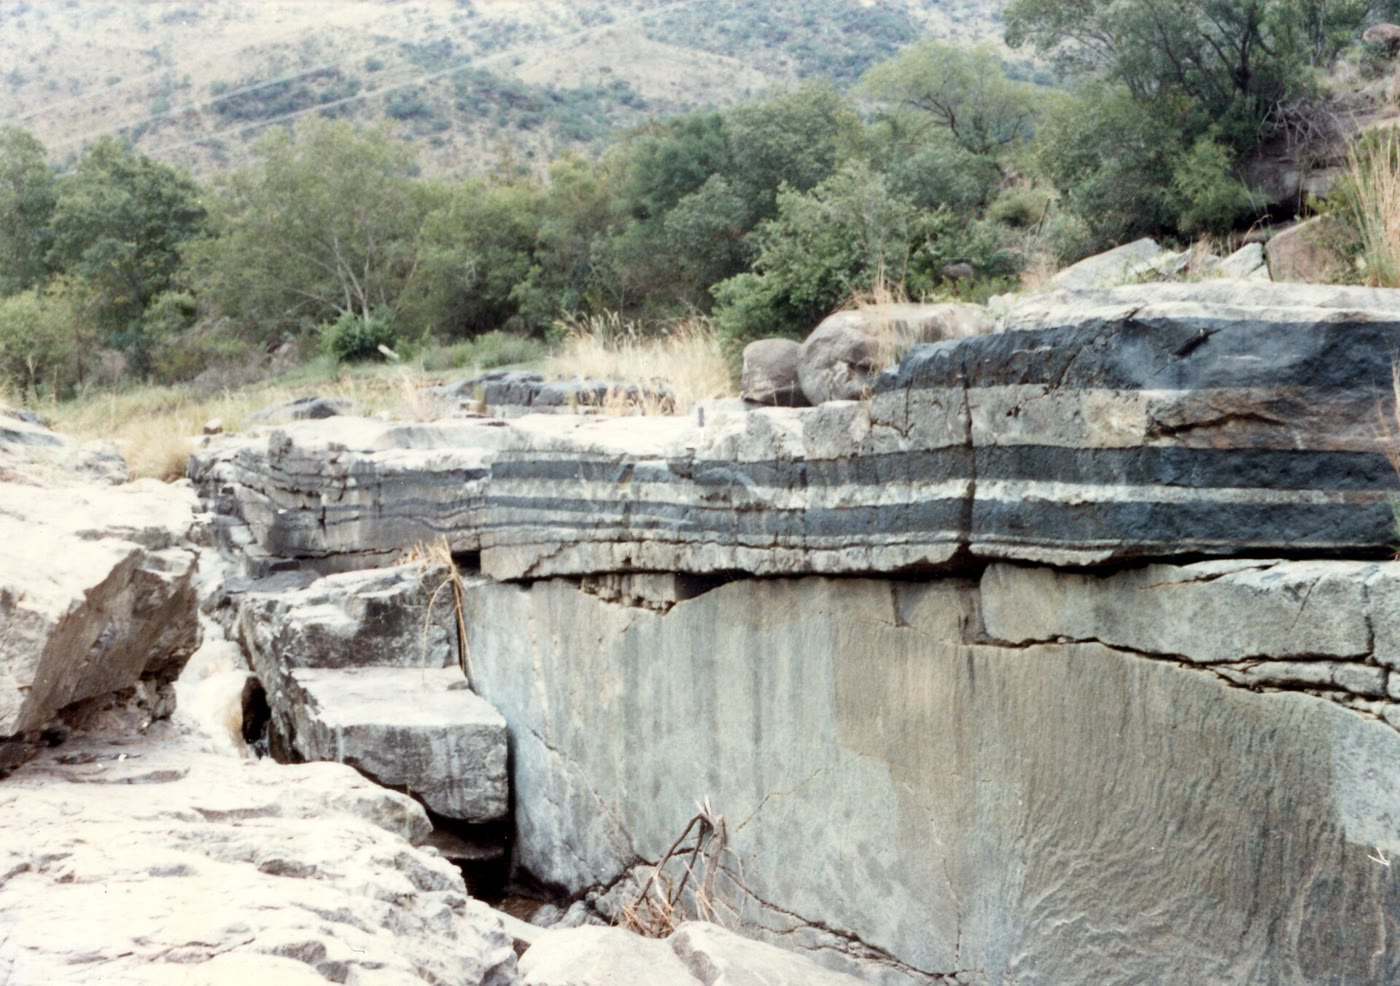
\includegraphics[height=5.2cm]{images/book4/b2-bushveld-chromitite.jpg}
\end{minipage}\hfill
\begin{minipage}[t]{0.42\linewidth}\vspace{0pt}\centering
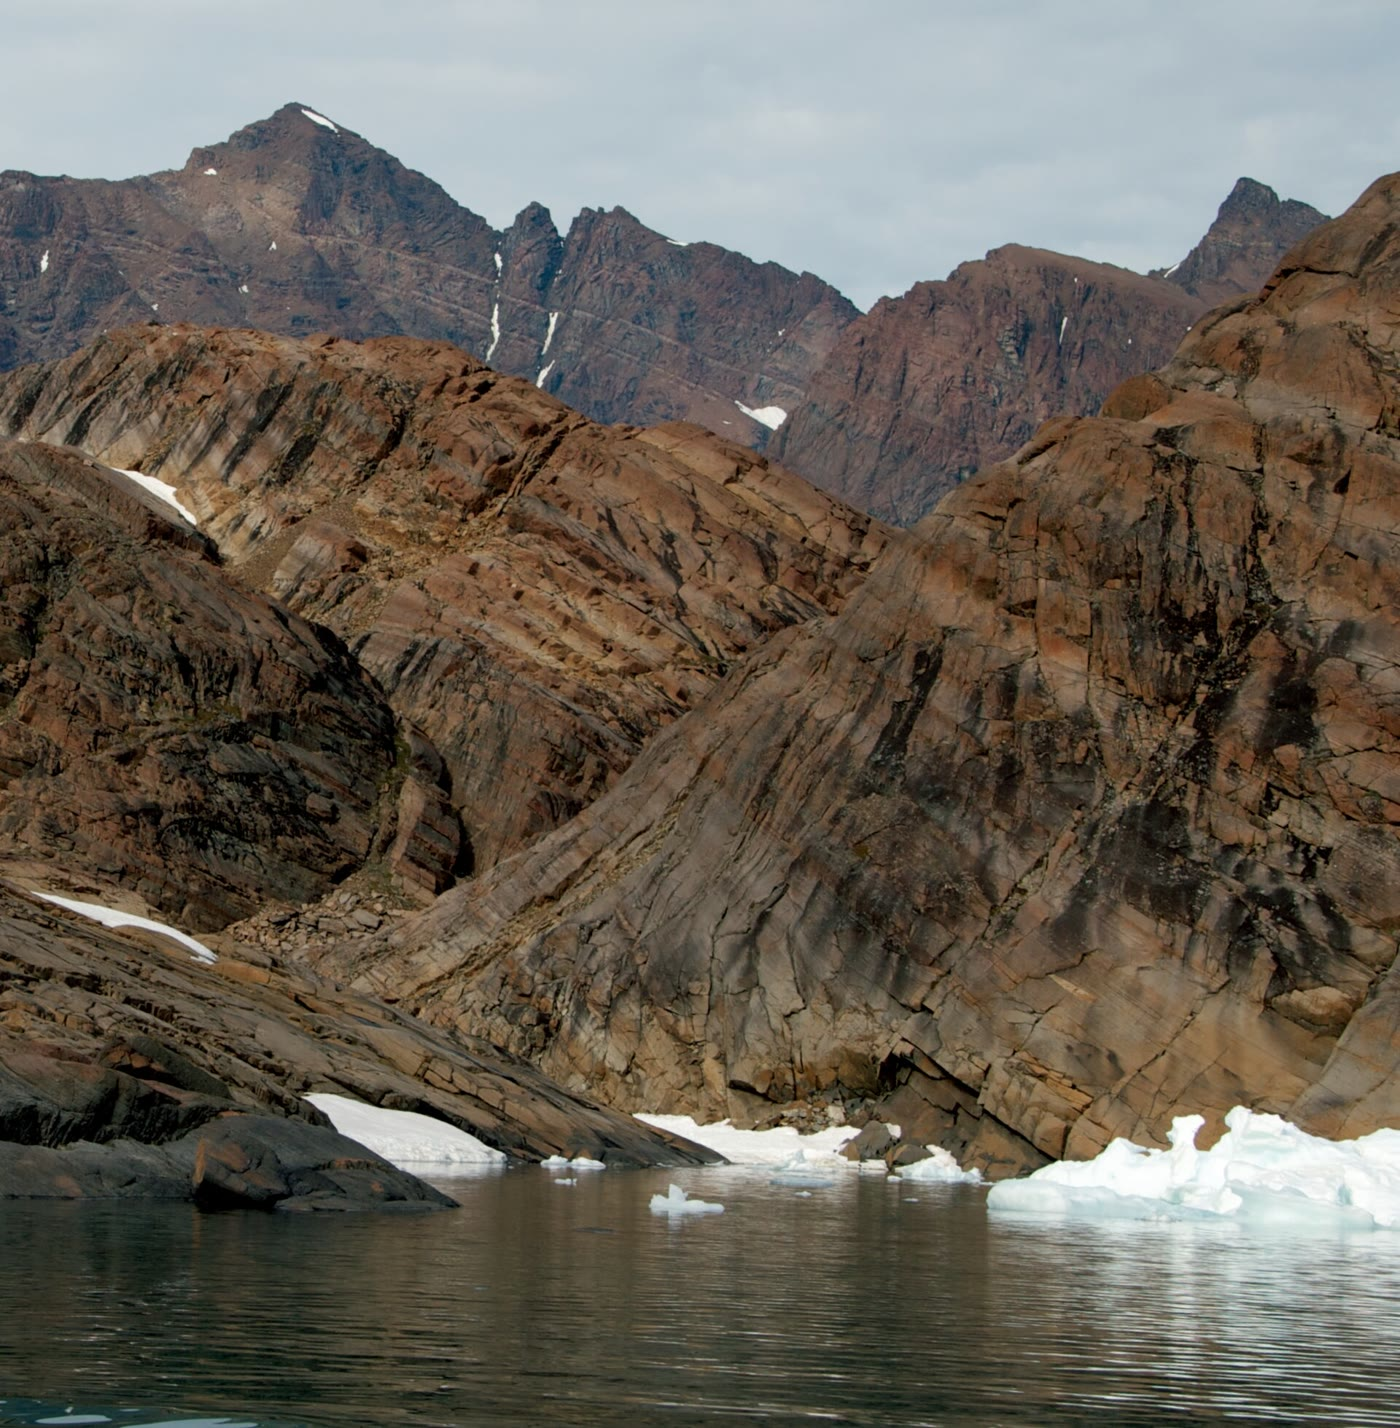
\includegraphics[height=5.2cm]{images/book4/b2-skaergaard-layering.jpg}
\end{minipage}
\par\smallskip{\small Kiri: lapisan kromitit hitam dan anortosit kelabu dari
Zona Kritis di Kompleks Bushveld, Afrika Selatan (Kevin Walsh, CC BY 2.0).
Kanan: gabro berlapis Zona Tengah intrusi Skaergaard, Greenland
Timur, yang miring dari kiri atas ke kanan bawah (C. Tegner, CC BY 4.0).}
\end{omfigure}

\section{Sistem terbuka}\label{sec:b2:magmatic-differentiation:open}

Dapur \omterm{def:b2:magma-emplacement:magma}{magma} jarang tertutup. \omterm{def:b2:magma-emplacement:magma}{Magma} baru datang dari bawah, dan dinding
dapur \omterm{def:b2:magma-emplacement:magma}{magma} adalah batuan yang dapat dipanaskan, dilelehkan, dan dilarutkan oleh \omterm{def:b2:magma-emplacement:magma}{magma}.

\begin{definition}[Pencampuran magma; asimilasi kerak; AFC]
\label{def:b2:magmatic-differentiation:open}
Yang disebut \emph{pencampuran magma}\index{pencampuran magma} adalah penyatuan dua \omterm{def:b2:magma-emplacement:magma}{magma} yang
komposisinya berbeda menjadi satu. Yang disebut \emph{asimilasi kerak}\index{asimilasi kerak} adalah
penggabungan batuan kerak ke dalam \omterm{def:b2:magma-emplacement:magma}{magma}, melalui pelelehan dan pelarutan batuan
dinding atau blok yang jatuh ke dalamnya. Yang disebut \emph{asimilasi--kristalisasi
fraksional}\index{asimilasi--kristalisasi fraksional} (AFC) adalah gabungan
keduanya dalam satu dapur \omterm{def:b2:magma-emplacement:magma}{magma}: \omterm{def:b2:magma-emplacement:magma}{magma} mengkristal, dan kalor laten yang dilepaskan
melelehkan dan mengasimilasi batuan dinding.
\end{definition}

\begin{proposition}[Pencampuran bersifat linear dalam konsentrasi]\label{prop:b2:magmatic-differentiation:mixing}
Campuran yang terdiri atas fraksi massa $s$ \omterm{def:b2:magma-emplacement:magma}{magma} A dan $1-s$ \omterm{def:b2:magma-emplacement:magma}{magma} B memiliki setiap
konsentrasi $C = sC_A + (1-s)C_B$: pada diagram apa pun yang memplot satu konsentrasi terhadap
konsentrasi lain, campuran terletak pada ruas garis lurus dari A ke B, dan aturan tuas memberikan
$s$.
\end{proposition}

\begin{proof}
Setiap unsur kekal: $C(m_A + m_B) = m_AC_A + m_BC_B$; bagilah dengan $m_A + m_B$.
\end{proof}

Pencampuran dan penyingkiran kristal sama-sama menghasilkan garis lurus pada \omterm{def:b2:magmatic-differentiation:harker}{diagram Harker}; rasio
isotop dapat membedakan keduanya. Kristalisasi tidak mengubah rasio isotop, sedangkan
pencampuran dengan batuan yang rasionya berbeda mengubahnya, menyusuri hiperbola pada
\cref{ch:b2:isotope-geochemistry}. Karena itu kenaikan $^{87}$Sr/$^{86}$Sr seiring silika dalam
suatu rangkaian vulkanik adalah tanda asimilasi.

\begin{proposition}[Asimilasi disertai kristalisasi fraksional]
\label{prop:b2:magmatic-differentiation:afc}
\omterm{def:b2:magma-emplacement:magma}{Magma} mengkristalkan kristal dengan koefisien partisi total $D$ untuk suatu unsur
dan mengasimilasi batuan dinding berkonsentrasi $C_a$ dengan laju $r$ kali laju
kristalisasi ($r \ne 1$). Dengan $F$ massa \omterm{def:b2:magma-emplacement:magma}{magma} relatif terhadap
massa awalnya dan $z = (r + D - 1)/(r - 1)$,
\[
\frac{C}{C_0} = F^{-z} + \frac{r}{r - 1 + D}\,\frac{C_a}{C_0}\,\bigl(1 - F^{-z}\bigr).
\]
Untuk $r = 0$, rumus ini adalah hukum Rayleigh. Rasio isotop unsur itu dalam \omterm{def:b2:magma-emplacement:magma}{magma}
adalah rata-rata rasio \omterm{def:b2:magma-emplacement:magma}{magma} awal dan rasio batuan dinding, yang diberi bobot oleh
kedua suku penjumlahan ini.
\end{proposition}

\begin{proof}
Per satuan massa awal, ketika massa $\mathrm dm_c$ mengkristal, massa
$r\,\mathrm dm_c$ terasimilasi dan massa \omterm{def:b2:magma-emplacement:magma}{magma} berubah sebesar $\mathrm dM =
-(1-r)\,\mathrm dm_c$. Neraca unsur itu adalah $\mathrm d(MC) = rC_a\,\mathrm dm_c -
DC\,\mathrm dm_c$. Dengan menjabarkan ruas kiri dan mengganti $\mathrm dm_c$ dengan
$-\mathrm dM/(1-r)$,
\[
M\frac{\mathrm dC}{\mathrm dM} = -C - \frac{rC_a - DC}{1-r}
= \frac{(r - 1 + D)\,C - rC_a}{1 - r} = -z\,\bigl(C - C^*\bigr),
\qquad C^* = \frac{rC_a}{r - 1 + D}.
\]
Jadi $\mathrm d(C - C^*)/(C - C^*) = -z\,\mathrm dM/M$, dan $C - C^*$ sebanding
dengan $M^{-z}$; dengan $C = C_0$ pada $M = 1$, $C = C^* + (C_0 - C^*)F^{-z}$, yaitu
rumus tersebut. Untuk $r = 0$, $z = 1 - D$ dan $C^* = 0$. Atom-atom yang berasal dari
\omterm{def:b2:magma-emplacement:magma}{magma} awal mematuhi persamaan yang sama dengan $C_a = 0$, sehingga konsentrasinya
$C_0F^{-z}$; sisanya berasal dari dinding: dari situlah pembobotan rasio isotop itu.
\end{proof}

DePaolo memberikan persamaan-persamaan ini pada 1981, dan persamaan itu menjadi model baku bagi \omterm{def:b2:magma-emplacement:magma}{magma}
yang terkontaminasi dalam perjalanannya menembus kerak. Persamaan itu menyembunyikan kendala termal. Kalor
untuk mengasimilasi batuan berasal dari kalor laten kristal: memanaskan kerak dari
150 sampai \qty{1150}{\celsius} memerlukan sekitar \qty{1}{kJ/g}, melelehkannya \qty{300}{J/g},
sedangkan \omterm{def:b2:magma-emplacement:magma}{magma} yang mengkristal memberikan sekitar \qty{400}{J/g}; jadi sekitar \qty{3.25}{g}
\omterm{def:b2:magma-emplacement:magma}{magma} harus mengkristal untuk setiap gram batuan yang terasimilasi, dan $r$ jauh di bawah 1.
Wilcox melakukan perhitungan yang sama untuk Parícutin: \qty{25.4}{g} monzonit
kuarsanya, yang diambil pada sekitar \qty{200}{\celsius}, memerlukan sekitar \qty{31350}{J} untuk
dipanaskan sampai \qty{1100}{\celsius} dan dilelehkan, yaitu kalor dari kristalisasi sekitar
\qty{85}{g} plagioklas, jauh lebih banyak daripada \qty{12.5}{g} kristal yang disingkirkan oleh neraca
massanya. \omterm{def:b2:magma-emplacement:magma}{Magma} yang meletus tidak mungkin membayar sendiri asimilasinya:
kalor itu pasti berasal dari tubuh \omterm{def:b2:magma-emplacement:magma}{magma} yang lebih besar daripada yang meletus, yang
mengkristal tanpa terlihat (\cref{exo:b2:magmatic-differentiation:11}).
% ledger: depaolo81:afc, white09:afc-heat, wilcox54:heat, wilcox54:mass-balance

\begin{omfigure}
\centering
\begin{tikzpicture}
\begin{axis}[omrecord, name=left, width=0.47\linewidth, height=5.4cm,
  xmin=0.3, xmax=1, ymin=0.3, ymax=1.05, x dir=reverse,
  xlabel={magma yang tersisa $F$}, ylabel={Sr: $C/C_0$},
  tick label style={font=\scriptsize}, label style={font=\small}]
\addplot[thick, black] table[x=F, y=srC_r0] {figdata/out/bachelor-2-differentiation-afc.dat};
\addplot[thick, blue!70!black] table[x=F, y=srC_r02] {figdata/out/bachelor-2-differentiation-afc.dat};
\addplot[thick, red!70!black] table[x=F, y=srC_r05] {figdata/out/bachelor-2-differentiation-afc.dat};
\end{axis}
\begin{axis}[omrecord, at={(left.east)}, anchor=west, xshift=1.7cm,
  width=0.47\linewidth, height=5.4cm,
  xmin=0.3, xmax=1, ymin=0.703, ymax=0.716, x dir=reverse,
  xlabel={magma yang tersisa $F$}, ylabel={$^{87}$Sr/$^{86}$Sr},
  y tick label style={/pgf/number format/fixed, /pgf/number format/precision=3},
  legend style={font=\scriptsize, at={(0.03,0.97)}, anchor=north west},
  tick label style={font=\scriptsize}, label style={font=\small}]
\addplot[thick, black] table[x=F, y=iso_r0] {figdata/out/bachelor-2-differentiation-afc.dat};
\addlegendentry{$r = 0$}
\addplot[thick, blue!70!black] table[x=F, y=iso_r02] {figdata/out/bachelor-2-differentiation-afc.dat};
\addlegendentry{$r = 0.2$}
\addplot[thick, red!70!black] table[x=F, y=iso_r05] {figdata/out/bachelor-2-differentiation-afc.dat};
\addlegendentry{$r = 0.5$}
\end{axis}
\end{tikzpicture}
\par\smallskip{\small Asimilasi disertai \omterm{def:b2:magmatic-differentiation:crystallisation}{kristalisasi fraksional} untuk stronsium
($D = 1.5$, batuan dinding dengan stronsium separuh stronsium \omterm{def:b2:magma-emplacement:magma}{magma} dan
$^{87}$Sr/$^{86}$Sr = 0.7200, \omterm{def:b2:magma-emplacement:magma}{magma} 0.7035; nilai ilustratif). Kiri:
konsentrasi turun makin cepat bila laju asimilasi $r$ makin besar, karena batuan dinding membawa
lebih sedikit stronsium dan lebih banyak kristal terbentuk untuk $F$ yang sama. Kanan: rasio
isotop, yang tidak diubah oleh kristalisasi saja ($r = 0$), naik menuju rasio dinding.}
\end{omfigure}

\section{Membaca kristal berzona}\label{sec:b2:magmatic-differentiation:zoning}

\begin{definition}[Zonasi komposisi]\label{def:b2:magmatic-differentiation:zoning}
Sebuah kristal larutan padat menunjukkan \emph{zonasi komposisi}\index{zonasi komposisi}
bila komposisinya berubah dari inti ke tepi, yang merekam perubahan cairan
tempat lapisan-lapisan berikutnya tumbuh. Zonasi disebut \emph{normal} bila tepinya lebih kaya akan
komponen bersuhu rendah (natrium pada plagioklas), \emph{terbalik} bila tepinya
lebih kaya akan komponen bersuhu tinggi, dan \emph{osilatori} bila keduanya berselang-seling.
\end{definition}

Kristal berzona adalah \omterm{def:b2:magmatic-differentiation:crystallisation}{kristalisasi fraksional} yang tertangkap basah: intinya tidak
menyesuaikan diri lagi dengan cairan yang datang kemudian. Gambar di bawah menghitung, pada lengkung Bowen,
plagioklas yang tumbuh dari cairan dengan \qty{50}{\percent} anortit. Pada
kesetimbangan, kristal tetap homogen dan berakhir pada \qty{50}{\percent}; pada \omterm{def:b2:magmatic-differentiation:crystallisation}{kristalisasi
fraksional} sempurna, setiap lapisan baru setimbang dengan cairan yang makin kaya natrium,
dan tepi kristal terakhir hampir berupa albit murni. Zonasi normal, dari
inti kalsik ke tepi natrik, adalah yang diramalkan seri Bowen bagi \omterm{def:b2:magma-emplacement:magma}{magma} yang mendingin. Zona
terbalik, yaitu pita kalsik di luar pita natrik, menunjukkan bahwa kristal itu tiba-tiba terendam dalam
cairan yang lebih panas atau lebih kalsik: sering kali kedatangan \omterm{def:b2:magma-emplacement:magma}{magma} baru, yaitu pencampuran di dalam
dapur \omterm{def:b2:magma-emplacement:magma}{magma}.
% ledger: bowen13:plagioclase, earle:bowen (Book 2)

\begin{omfigure}
\centering
\begin{tikzpicture}
\begin{axis}[omrecord, width=0.78\linewidth, height=6cm,
  xmin=0, xmax=1, ymin=0, ymax=90,
  xlabel={fraksi cairan yang telah mengkristal},
  ylabel={anortit (\unit{\percent}, molekuler)},
  legend style={font=\scriptsize, at={(0.02,0.02)}, anchor=south west},
  tick label style={font=\scriptsize}, label style={font=\small}]
\addplot[very thick, red!70!black] table[x=x, y=an_frac] {figdata/out/bachelor-2-differentiation-zoning.dat};
\addlegendentry{fraksional: lapisan yang terbentuk}
\addplot[thick, gray, densely dotted] table[x=x, y=an_liq_frac] {figdata/out/bachelor-2-differentiation-zoning.dat};
\addlegendentry{fraksional: cairan}
\addplot[very thick, blue!70!black, dashed] table[x=x, y=an_eq] {figdata/out/bachelor-2-differentiation-zoning.dat};
\addlegendentry{setimbang: kristal}
\end{axis}
\end{tikzpicture}
\par\smallskip{\small Plagioklas yang mengkristal dari cairan dengan \qty{50}{\percent}
anortit, dihitung pada lengkung Bowen (1913). Pada \omterm{def:b2:magmatic-differentiation:crystallisation}{kristalisasi fraksional},
lapisan-lapisan kristal yang berurutan, dari inti (kiri) ke tepi (kanan), makin kaya
natrium, dan cairan mencapai albit ketika sekitar \qty{82}{\percent} telah mengkristal; pada
\omterm{def:b2:magmatic-differentiation:crystallisation}{kristalisasi setimbang}, kristal tetap seragam dan berakhir dengan komposisi
cairan asalnya.}
\end{omfigure}

\begin{inthelab}[Membaca kristal berzona]
Ahli petrologi mula-mula membaca zonasi di antara polarisator bersilang, tempat zona-zona
plagioklas padam pada sudut yang sedikit berbeda dan tampak sebagai pita-pita konsentris.
Kemudian mereka mengukurnya: mikroprobe elektron (\cref{ch:b2:field-lab-methods-2})
menganalisis titik-titik selebar beberapa mikrometer di sepanjang lintasan dari inti ke tepi, dan peta
kalsium dan natrium memperlihatkan zona-zona itu secara langsung. Dari profil semacam itu mereka menghitung
komposisi cairan tempat setiap zona tumbuh, dengan lengkung pada gambar di atas atau
dengan koefisien partisi, dan mereka menghitung zona terbalik sebagai banyaknya
pengisian ulang dapur \omterm{def:b2:magma-emplacement:magma}{magma}. \omterm{def:b2:elements-in-the-earth:trace}{Unsur jejak} yang diukur di sepanjang lintasan yang sama dengan ablasi
laser, dan rasio isotop yang diukur zona demi zona, memisahkan kristalisasi, pencampuran,
dan asimilasi dalam sejarah satu kristal.
\end{inthelab}

\section{Latihan}

\begin{exercise}[$\star$]\label{exo:b2:magmatic-differentiation:1}
Gunakan hasil pengukuran Bowen pada plagioklas (solidus / likuidus, \unit{\celsius}):
An$_{100}$ 1550 / 1550; An$_{83.3}$ 1465 / 1521; An$_{66.7}$ 1372 / 1490; An$_{50}$
1287 / 1450; An$_{33.3}$ 1205 / 1394; An$_{20}$ likuidus 1334; An$_{11.1}$ likuidus
1265, dan lakukan interpolasi linear di antara titik-titik yang bertetangga. Cairan dengan
\qty{50}{\percent} anortit mendingin secara setimbang. (a) Pada suhu berapa cairan itu
mulai mengkristal, dan bagaimana komposisi kristal pertamanya? (b) Pada
\qty{1394}{\celsius}, bagaimana komposisi cairan dan kristal,
dan berapa fraksi massa yang telah mengkristal (gunakan fraksi mol seolah-olah fraksi
massa)? (c) Bagaimana komposisi tetes cairan terakhir?
\end{exercise}
% ledger: bowen13:plagioclase

\begin{exercise}[$\star$]\label{exo:b2:magmatic-differentiation:2}
Sebuah \omterm{def:b2:magmatic-differentiation:cumulate}{kumulat} gabroik mengandung \qty{50}{\percent} plagioklas, \qty{35}{\percent}
klinopiroksen, dan \qty{15}{\percent} olivin. Dengan koefisien partisi
(olivin / klinopiroksen / plagioklas) Sr 0.000063 / 0.157 / 2.7, Zr 0.00068 /
0.195 / 0.001, dan Rb 0.000044 / 0.0033 / 0.025, hitunglah koefisien partisi
total setiap unsur, dan sebutkan mana yang kompatibel.
\end{exercise}
% ledger: white07:kd-basalt

\begin{exercise}[$\star$]\label{exo:b2:magmatic-differentiation:3}
\omterm{def:b2:magmatic-differentiation:cumulate}{Kumulat} pada \cref{exo:b2:magmatic-differentiation:2} mengkristal dari basal melalui \omterm{def:b2:magmatic-differentiation:crystallisation}{kristalisasi fraksional}
sampai cairannya tersisa separuh. (a) Dengan faktor berapa Sr, Zr, dan Rb masing-masing berubah
dalam cairan (ambillah koefisien total 1.40, 0.069, dan 0.014)? (b) Dengan faktor berapa
rasio Zr/Rb berubah? Berilah komentar dengan memakai korolari tentang rasio.
\end{exercise}
% ledger: white07:kd-basalt

\begin{exercise}[$\star$]\label{exo:b2:magmatic-differentiation:4}
Lava pertama Parícutin (Februari 1943) mengandung \qty{55.04}{\percent} \ce{SiO2},
\qty{5.68}{\percent} \ce{MgO}, dan \qty{0.85}{\percent} \ce{K2O}; lava terakhir (Februari
1952), 60.07, 3.73, dan \qty{1.67}{\percent}. (a) Hitunglah perubahan setiap oksida.
(b) Kalium oksida tidak masuk ke mineral mana pun yang mengkristal. Seandainya oksida itu dipekatkan oleh
\omterm{def:b2:magmatic-differentiation:crystallisation}{kristalisasi fraksional} saja, berapa fraksi cairan yang akan tersisa?
(c) Neraca massa Wilcox hanya menyingkirkan sekitar \qty{12.5}{g} kristal per
\qty{100}{g} \omterm{def:b2:magma-emplacement:magma}{magma}. Apa yang ditunjukkan oleh perbandingan itu?
\end{exercise}
% ledger: wilcox54:table2, wilcox54:mass-balance

\begin{exercise}[$\star\star$]\label{exo:b2:magmatic-differentiation:5}
Bandingkan \omterm{def:b2:magmatic-differentiation:crystallisation}{kristalisasi fraksional} dan \omterm{def:b2:magmatic-differentiation:crystallisation}{kristalisasi setimbang}: hitunglah $C_L/C_0$ dengan kedua hukum
(a) untuk nikel, $D = 5$, ketika \qty{20}{\percent} cairan telah mengkristal; (b)
untuk \omterm{def:b2:elements-in-the-earth:partition}{unsur inkompatibel}, $D = 0.01$, ketika \qty{90}{\percent} telah mengkristal.
(c) Berapa limit kedua hukum itu ketika $F \to 0$? Hukum mana yang dapat melucuti suatu
\omterm{def:b2:elements-in-the-earth:partition}{unsur kompatibel} dari cairan sepenuhnya?
\end{exercise}

\begin{exercise}[$\star\star$]\label{exo:b2:magmatic-differentiation:6}
(a) Hitunglah persentase massa \ce{MgO}, \ce{FeO}, dan \ce{SiO2} dalam olivin
Fo$_{80}$, $(\ce{Mg}_{0.8}\ce{Fe}_{0.2})_2\ce{SiO4}$ ($M$ = 40.30, 71.84, dan
\qty{60.08}{g/mol}). (b) Sebuah basal dengan \qty{10.0}{\percent} \ce{MgO} dan
\qty{49.0}{\percent} \ce{SiO2} hanya mengkristalkan olivin ini sampai cairannya mengandung
\qty{8.0}{\percent} \ce{MgO}. Berapa fraksi massa olivin yang tersingkir? (c) Berapa
kadar silika cairan saat itu?
\end{exercise}

\begin{exercise}[$\star\star$]\label{exo:b2:magmatic-differentiation:7}
Untuk intrusi Skaergaard, $F = \num{1.091e-7}H^2 - \num{5.9064e-4}H + 0.7678$.
(a) Hitunglah $F$ pada $H = 0$, 1000, dan \qty{2000}{m}. (b) Pada ketinggian berapa $F = 0$?
(c) Berapa fraksi \omterm{def:b2:magma-emplacement:magma}{magma} yang telah mengkristal sebelum dasar urutan lantai yang tersingkap
terbentuk, dan di mana bagian itu mungkin berada?
\end{exercise}
% ledger: tegner23:skaergaard

\begin{exercise}[$\star\star$]\label{exo:b2:magmatic-differentiation:8}
Di sepanjang penampang Skaergaard, \omterm{def:b2:magmatic-differentiation:cumulate}{kumulat} median mengandung \qty{177}{ppm} Ni pada
$F = 0.70$ (Zona Bawah a), \qty{54}{ppm} pada $F = 0.29$ (Zona Tengah), dan
\qty{6.2}{ppm} pada $F = 0.17$ (Zona Atas a). (a) Dengan menganggap bahwa \omterm{def:b2:magmatic-differentiation:cumulate}{kumulat} mengandung nikel
$D$ kali nikel cairannya dan bahwa cairan mengikuti hukum Rayleigh,
hitunglah $D$ semu antara dua tingkat pertama. (b) Lakukan hal yang sama antara
dua tingkat terakhir. (c) Apa yang dapat membuat $D$ semu berubah?
\end{exercise}
% ledger: data:b4-skaergaard

\begin{exercise}[$\star\star$]\label{exo:b2:magmatic-differentiation:9}
Periksalah jawaban Wilcox: \qty{100}{g} massa dasar lava pertama (\ce{SiO2}
55.53, \ce{MgO} 4.66, \ce{K2O} \qty{0.88}{\percent}) ditambah \qty{25.4}{g} xenolit
rata-rata (72.48, 0.77, 3.64) dikurangi \qty{2.9}{g} olivin Fo$_{80}$ (39.19, 42.06, 0)
dikurangi \qty{9.6}{g} plagioklas An$_{70}$ (50.54, 0, 0). (a) Berapa massa yang tersisa?
(b) Hitunglah \ce{SiO2}, \ce{MgO}, dan \ce{K2O}-nya dan bandingkan dengan massa dasar
lava 19 (60.16, 3.19, dan \qty{1.75}{\percent}). (c) Oksida mana yang paling tidak cocok?
\end{exercise}
% ledger: wilcox54:groundmass, wilcox54:xenoliths, wilcox54:mass-balance

\begin{exercise}[$\star\star\star$]\label{exo:b2:magmatic-differentiation:10}
Sebuah \omterm{def:b2:magma-emplacement:magma}{magma} mengasimilasi batuan dinding dengan $r = 0.2$ sambil mengkristal, dengan $D_{\ce{Sr}} =
1.5$, $C_a/C_0 = 0.5$, $^{87}$Sr/$^{86}$Sr awal = 0.7035, dan batuan dinding 0.7200.
(a) Hitunglah $z$, $F^{-z}$, dan $C/C_0$ pada $F = 0.7$. (b) Bandingkan dengan \omterm{def:b2:magmatic-differentiation:crystallisation}{kristalisasi
fraksional} murni pada $F$ yang sama, dan jelaskan perbedaannya dengan massa kristal
yang terbentuk dalam setiap kasus. (c) Hitunglah $^{87}$Sr/$^{86}$Sr \omterm{def:b2:magma-emplacement:magma}{magma} itu.
\end{exercise}

\begin{exercise}[$\star\star\star$]\label{exo:b2:magmatic-differentiation:11}
Ikutilah neraca kalor Wilcox untuk Parícutin. (a) Berapa kalor yang diperlukan satu gram monzonit
kuarsa untuk naik dari 200 ke \qty{1100}{\celsius} (kapasitas kalor
\qty{1.1}{J/(g.K)}) lalu meleleh (\qty{250}{J/g})? (b) Berapa untuk
\qty{25.4}{g}? (c) Berapa massa plagioklas An$_{70}$ (kalor laten \qty{370}{J/g})
yang harus mengkristal untuk memasoknya? (d) Bandingkan dengan \qty{12.5}{g} kristal pada
neraca massa, hitunglah rasio $r$ asimilasi terhadap kristalisasi, dan sebutkan apa
artinya.
\end{exercise}
% ledger: wilcox54:heat, white09:afc-heat

\begin{exercise}[$\star\star\star$]\label{exo:b2:magmatic-differentiation:12}
Sebuah basal dengan \qty{250}{ppm} Ni mula-mula mengkristalkan olivin saja ($D = 5$) sampai
$F = 0.8$, lalu olivin bersama plagioklas dan klinopiroksen (koefisien total $D = 1.5$). (a)
Hitunglah faktor perubahan nikel pada setiap tahap, dan kadar nikel
cairan pada $F = 0.5$. (b) Apa yang akan diramalkan oleh satu hukum dengan $D = 5$?
(c) Jelaskan mengapa hukum Rayleigh harus diterapkan secara bertahap.
\end{exercise}

\section{Soal: Intrusi yang menulis sejarahnya sendiri}

\begin{problem}[{Soal akhir pekan --- dari lapisan-lapisan sebuah gabro sampai fraksi
magmanya yang masih cair pada akhirnya}]
\label{pb:b2:magmatic-differentiation:1}
Sebuah \omterm{def:b2:magma-emplacement:bodies}{sill} gabro berlapis (rekaan) mengkristal dari basal yang \omterm{def:b2:magma-emplacement:aureole}{tepi dinginnya}
memberikan komposisi induk: \ce{SiO2} 49.5, \ce{Al2O3} 16.0, \ce{FeO} 10.0,
\ce{MgO} 9.0, \ce{CaO} 11.5, \ce{Na2O} 2.5, \ce{K2O} \qty{0.30}{\percent};
\qty{150}{ppm} Ni dan \qty{80}{ppm} Zr. \omterm{def:b2:magmatic-differentiation:cumulate}{Kumulat} zona bawah terdiri atas
\qty{20}{\percent} olivin, \qty{50}{\percent} plagioklas, dan \qty{30}{\percent}
klinopiroksen; di atas tingkat tempat olivin menghilang, \omterm{def:b2:magmatic-differentiation:cumulate}{kumulat} terdiri atas \qty{55}{\percent}
plagioklas dan \qty{45}{\percent} klinopiroksen. Ambillah koefisien partisi
(olivin / plagioklas / klinopiroksen) Ni 5.0 / 0 / 2.0 dan Zr 0.0007 / 0.001 /
0.195. Komposisi mineral (\unit{\percent}): olivin \ce{MgO} 42.06, \ce{CaO} 0,
\ce{Al2O3} 0, \ce{SiO2} 39.19; plagioklas 0, 14.36, 31.70, 50.54; klinopiroksen
16.0, 20.5, 3.0, 51.5. Sebuah \omterm{def:b2:magma-emplacement:bodies}{retas}
batuan berbutir halus yang dipasok dari dapur \omterm{def:b2:magma-emplacement:magma}{magma} ketika lapisan teratas mengkristal mengandung
\ce{SiO2} 50.0, \ce{Al2O3} 14.1, \ce{FeO} 16.7, \ce{MgO} 4.9, \ce{CaO} 7.3,
\ce{Na2O} 3.4, \ce{K2O} \qty{0.75}{\percent}, dan \qty{188}{ppm} Zr.

\noindent\textbf{Bagian I --- Koefisien partisi lapisan-lapisan.}
\begin{enumerate}
\item Hitunglah koefisien partisi total nikel di zona bawah.
\item Hitunglah koefisien partisi total zirkonium di zona bawah.
\item Hitunglah keduanya di zona atas.
\item Unsur mana yang kompatibel di setiap zona? Apakah nikel tetap kompatibel ketika
olivin menghilang?
\item Mineral mana yang menyimpan sebagian besar zirkonium \omterm{def:b2:magmatic-differentiation:cumulate}{kumulat}, dan mengapa?
\item Dengan faktor berapa Ni/Zr dalam cairan berubah setiap kali $F$ menjadi separuhnya di zona
bawah?
\end{enumerate}

\noindent\textbf{Bagian II --- Kurva Rayleigh di sepanjang penampang.}
\begin{enumerate}[resume]
\item Berapa kadar nikel yang kamu harapkan dalam \omterm{def:b2:magmatic-differentiation:cumulate}{kumulat} terbawah, yang mengkristal pada
$F = 1$?
\item Sebuah \omterm{def:b2:magmatic-differentiation:cumulate}{kumulat} zona bawah yang lebih tinggi mengandung \qty{190}{ppm} Ni. Pada $F$ berapa \omterm{def:b2:magmatic-differentiation:cumulate}{kumulat} itu
terbentuk?
\item Berapa kadar zirkonium cairan saat itu?
\item Pada $F$ itu, bandingkan nikel cairan yang diberikan oleh hukum fraksional dan hukum
setimbang.
\item Olivin menghilang pada $F = 0.55$. Hitunglah kadar nikel cairan
di sana.
\item Hitunglah nikel \omterm{def:b2:magmatic-differentiation:cumulate}{kumulat} yang terbentuk tepat di bawah dan tepat di atas tingkat
itu. Ciri apa yang akan dilihat ahli geologi pada profilnya?
\item Hitunglah nikel cairan dan \omterm{def:b2:magmatic-differentiation:cumulate}{kumulat} pada $F = 0.40$. Jelaskan
trennya.
\end{enumerate}

\noindent\textbf{Bagian III --- Neraca massa cairan terakhir.}
\begin{enumerate}[resume]
\item Tuliskan persamaan kekekalan menurut metode itu untuk satu oksida, dengan massa
$x_{\mathrm{ol}}, x_{\mathrm{pl}}, x_{\mathrm{cpx}}$ yang tersingkir per \qty{100}{g}
\omterm{def:b2:magma-emplacement:magma}{magma} induk dan \omterm{def:b2:magma-emplacement:bodies}{retas} itu sebagai cairan turunan.
\item Tuliskan persamaan itu untuk \ce{MgO}, \ce{CaO}, dan \ce{Al2O3}.
\item Selesaikan sistem $3 \times 3$ itu.
\item Berapa fraksi \omterm{def:b2:magma-emplacement:magma}{magma} induk yang tersisa sebagai cairan?
\item Periksalah jawabanmu dengan \ce{SiO2}: hitung ulang silika cairan dari
massa yang diperoleh.
\item Bandingkan proporsi mineral yang tersingkir dengan komposisi modal kedua
zona.
\item Kalium oksida tidak masuk ke mineral mana pun: berapa fraksi cairan yang diberikannya?
\end{enumerate}

\noindent\textbf{Bagian IV --- Fraksi cairan di puncak.}
\begin{enumerate}[resume]
\item Dengan faktor berapa zirkonium telah naik dalam cairan ketika olivin menghilang pada
$F = 0.55$? Berikan kadar zirkonium saat itu.
\item Dari zirkonium \omterm{def:b2:magma-emplacement:bodies}{retas}, hitunglah fraksi cairan yang tersisa ketika \omterm{def:b2:magma-emplacement:bodies}{retas} itu
terbentuk, dengan menerapkan hukum zona atas mulai dari $F = 0.55$.
\item Ulangi perhitungan dengan satu nilai $D = 0.07$ sejak awal. Apakah jawabannya
peka terhadap rincian $D$?
\item Besi naik dari 10.0 menjadi \qty{16.7}{\percent} dalam cairan sementara silika hampir tidak
berubah. Mineral mana yang bertanggung jawab, dan seri magmatik jenis apa yang
dibayangkan oleh hal ini (\cref{ch:b2:magmatic-series})?
\item \omterm{def:b2:magmatic-differentiation:cumulate}{Kumulat} teratas mengandung \qty{47}{ppm} Zr. Kristal kumulus saja akan mengandung zirkonium
$\bar D$ kali zirkonium cairan; berapa fraksi massa cairan terperangkap
(berkomposisi seperti \omterm{def:b2:magma-emplacement:bodies}{retas} itu) yang menjelaskan hasil analisis tersebut?
\item Nyatakan fraksi \omterm{def:b2:magma-emplacement:magma}{magma} asal yang masih cair ketika lapisan teratas
mengkristal, yaitu angka kunci soal ini, dan bandingkan ketiga taksiran
(unsur utama, kalium oksida, zirkonium).
\end{enumerate}
\end{problem}
% ledger: white07:kd-basalt, matzen12:dni
